% Лабораторная работа по информатике № 1
% Михедов Константин Константинович БИБ224

%Тип документа: статья, размер бумаги - A4, написано 14 кегелем
\documentclass[a4paper,12pt]{article}

% Поиск по скомпилированному PDF
\usepackage{cmap}
% Кодировка выходного текста
\usepackage[T2A]{fontenc}
% Кодировка исходного текста
\usepackage[utf8]{inputenc}
% Поддержка необходимых языков
\usepackage[english,russian]{babel}

% Поддержка изображений
\usepackage{graphicx}
% Путь до внешних изображений
\graphicspath{ {./figures/}}

% Умная запятая
\usepackage{icomma}

% Ссылки на электронные ресурсы
\usepackage{hyperref}
% Настройка внешнего вида ссылок
\hypersetup{
  % Отключить прямоугольную рамку
  pdfborder={0 0 0},
  % Включить цветные ссылки
  colorlinks=true,
  % Цвет для ссылок на веб-ресурсы
  urlcolor=blue,
  % Цвет внутренних ссылок
  linkcolor=black
}

% Дополнительная математика
\usepackage{amsmath,amsfonts,amssymb,amsthm,mathtools}
% Показывать номера только у тех выржений, на которые кто-то ссылается
\mathtoolsset{showonlyrefs=true}

% Дополнительные символы
\usepackage{mathbbol}

% Правильное оформление
% Настройка отступов
\usepackage[left=2cm,right=1cm,top=2cm,bottom=2cm]{geometry}
% Настройка шрифта
\usepackage{fontspec}
\setmainfont{Times New Roman}
% Настройка межстрочных интервалов
\usepackage{setspace}
\onehalfspacing
% и межабзацных
\usepackage{parskip}
\setlength{\parindent}{1.25cm} 

% Красная строка
\usepackage{indentfirst}
\setlength{\parindent}{1.25cm} 

% Корректное положение рисунков?
\usepackage{float}

\begin{document}
  % Титульная страница
  \begin{titlepage}
    \begin{center}
      ФЕДЕРАЛЬНОЕ ГОСУДАРСТВЕННОЕ АВТОНОМНОЕ \\
      ОБРАЗОВАТЕЛЬНОЕ УЧРЕЖДЕНИЕ ВЫСШЕГО ОБРАЗОВАНИЯ \\
      <<НАЦИОНАЛЬНЫЙ ИССЛЕДОВАТЕЛЬСКИЙ УНИВЕРСИТЕТ \\
      <<ВЫСШАЯ ШКОЛА ЭКОНОМИКИ>>

      \textit{
        Московский институт электроники и математики им. А.Н.Тихонова
      }

      \vspace{4cm}

      \textbf{
        ЗНАКОМСТВО С САПР ALTERA QUARTUS II
      }

      \vspace{1.5cm}

      Практическая работа № 1\\
      по направлению 10.03.01 Информационная безопасность \\
      студента образовательной программы бакалавриата \\
      <<Информационная безопасность>>
    \end{center}

    \vspace{1.25cm}

    \begin{flushright}
        Проверил:

        $\underset{\text{И.О. Фамилия}}{\underline{\hspace{0.3\textwidth}}}$

        $\underset{\text{Подпись}}{\underline{\hspace{0.3\textwidth}}}$
    \end{flushright}

    \vspace{1.25cm}

    \begin{flushright}
        Выполнил:

        $\overset{\text{К.К. Михедов}}{\underset{\text{И.О. Фамилия}}{\underline{\hspace{0.3\textwidth}}}}$
        
        $\underset{\text{Подпись}}{\underline{\hspace{0.3\textwidth}}}$
    \end{flushright}

    \vfill

    \begin{center}
        Москва 2022 г.
    \end{center}
  \end{titlepage}

  %\section{Ход работы}

  \section{Часть 1}

  \paragraph{
    Составить схему указанного выражения в базисе И, ИЛИ, НЕ. Построить временную диаграмму
    и выполнить моделирование в режимах Functional и Time
  }

  Исходное выражения для 19 варианта: $F = \overline{c} \lor (n \land \overline{c})$. Построим
  для него таблицу истинности:

  \begin{table}[h]
	\centering
	\begin{tabular}{|c c | c c | c |}
		\hline
        c & n & $\overline{c}$ & $n \land \overline{c}$ & F \\
        \hline
        0 & 0 & 1 & 0 & 1 \\
        0 & 1 & 1 & 1 & 1 \\
        1 & 0 & 0 & 0 & 0 \\
        1 & 1 & 0 & 0 & 0 \\
        \hline      
    \end{tabular}
    \caption{Таблица истинности исходного выражения}
    \label{table:1}
  \end{table}

  Сразу же упростим исходное выражение с помощью алгебры логики: 
  $F = \overline{c} \lor (n \land \overline{c}) = \overline{c}$

  Приступим к моделированию логического выражения в САПР. Во-первых, необоходимо
  создать новый проект САПР Quartus II:

  \begin{figure}[H]
    \centering
    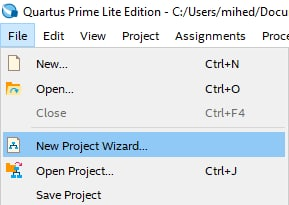
\includegraphics[width=5cm]{01_01}
    \caption{Выбираем команду \textbf{New Project Wizard...}}
  \end{figure}

  \begin{figure}[H]
    \centering
    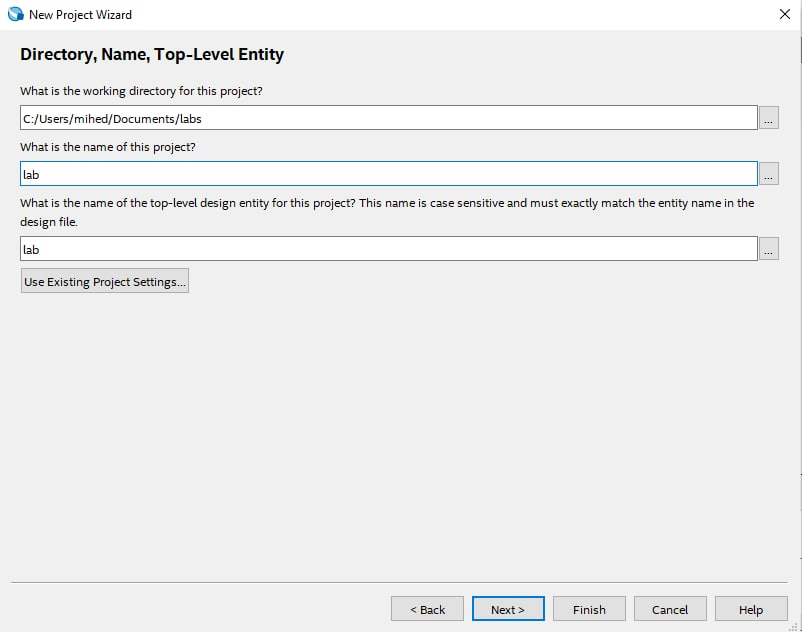
\includegraphics[width=9cm]{01_02}
    \caption{Указываем название проекта и его расположение}
  \end{figure}

  \begin{figure}[H]
    \centering
    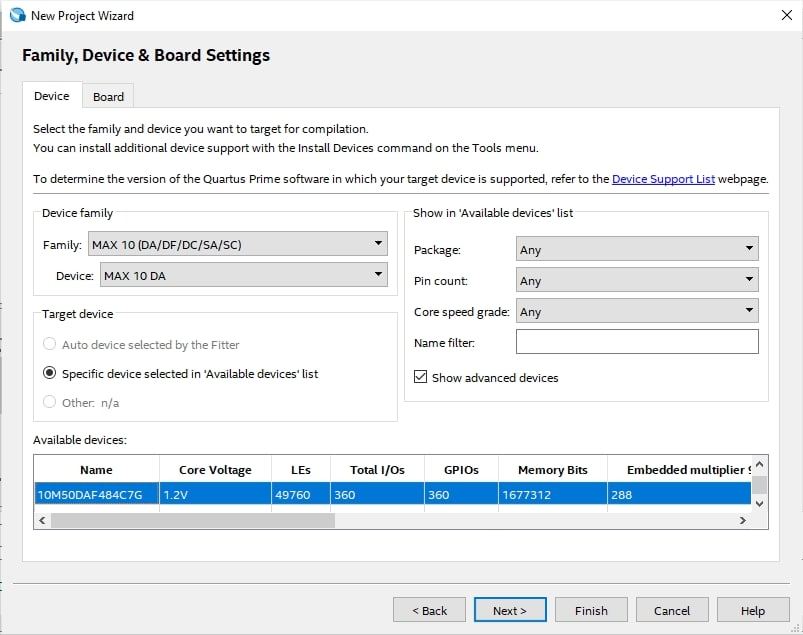
\includegraphics[width=9cm]{01_03}
    \caption{Подключаем поддержку необходимых устройств (в нашем случае 10M50DAF484C7G)}
  \end{figure}

  Завершаем настройку проекта нажатием на кнопку \textbf{Finish}.

  \begin{figure}[H]
    \centering
    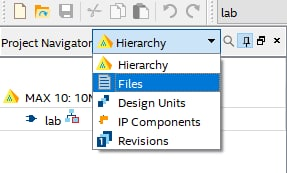
\includegraphics[width=5cm]{01_04}
    \caption{Для удобства указываем пофайловое отображение структуры проекта}
  \end{figure}

  \begin{figure}[H]
    \centering
    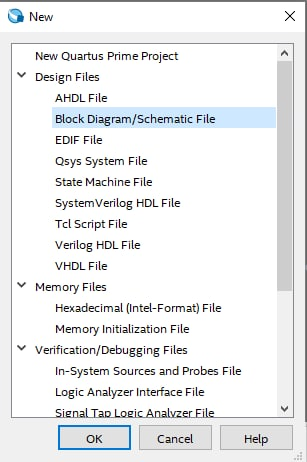
\includegraphics[width=4.5cm]{01_05}
    \caption{Создадим новый bdf файл}
  \end{figure}

  \begin{figure}[H]
    \centering
    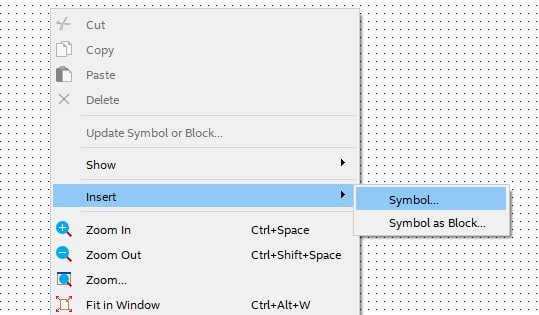
\includegraphics[width=6cm]{01_06}
    \caption{Откроем меню добавления логических элементов}
  \end{figure}

  \begin{figure}[H]
    \centering
    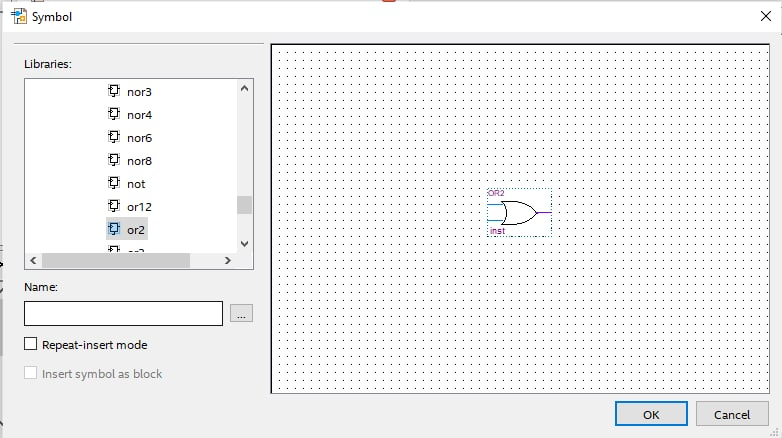
\includegraphics[width=9cm]{01_07}
    \caption{Выбираем необходимые элементы из списка}
  \end{figure}

  Для базовой схемы потребуется один элемент НЕ, один элемент ИЛИ и один элемент И, для упрощенной
  толькой один элемент НЕ. Также необходимо добавить 2 входа (для переменных c и n) и два выхода
  (один для базового выражения, другой - для упрощенного).

  \begin{figure}[H]
    \centering
    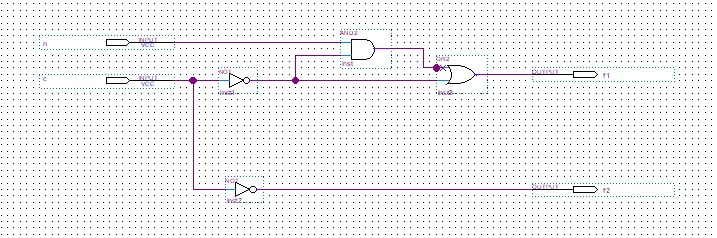
\includegraphics[width=10cm]{01_08}
    \caption{Построим схему обычного и упрощенного выражений}
  \end{figure}

  \begin{figure}[H]
    \centering
    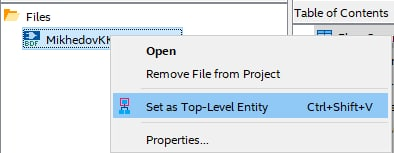
\includegraphics[width=6cm]{01_09}
    \caption{Установим текущую сборку в качестве основной}
  \end{figure}

  \begin{figure}[H]
    \centering
    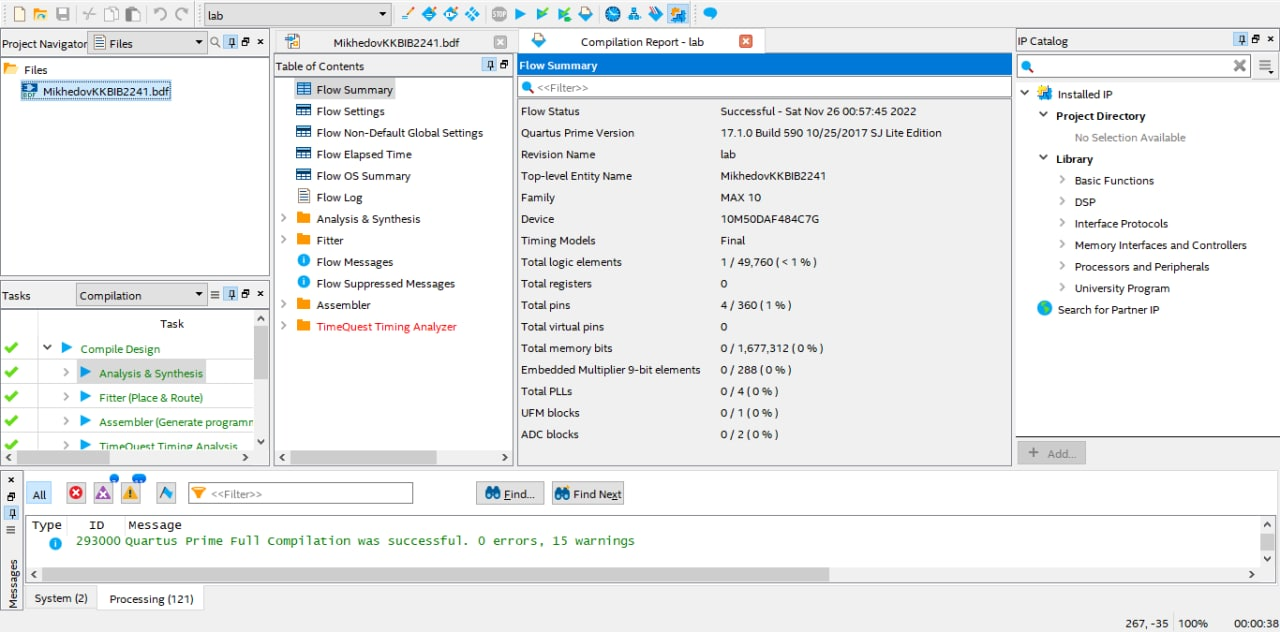
\includegraphics[width=12cm]{01_10}
    \caption{Выполним компиляцию проекта}
  \end{figure}

  \begin{figure}[H]
    \centering
    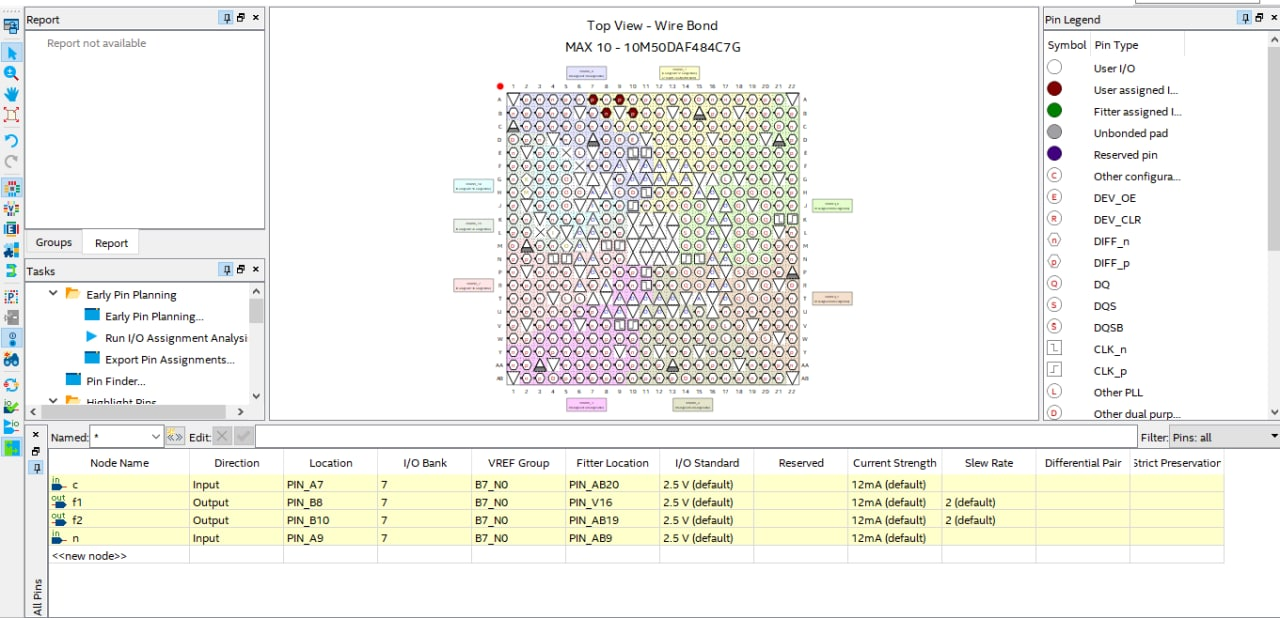
\includegraphics[width=12cm]{01_11}
    \caption{При помощи \textbf{Pin Planer} присвоим входам и выходам подходящие порты}
  \end{figure}

  \begin{figure}[H]
    \centering
    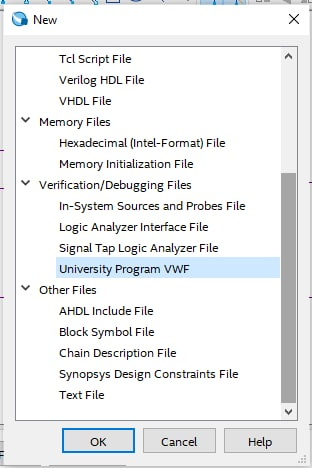
\includegraphics[width=4.5cm]{01_12}
    \caption{Создадим новый wvf файл}
  \end{figure}

  \begin{figure}[H]
    \centering
    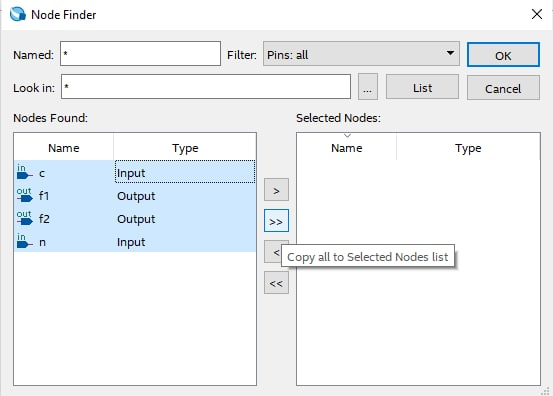
\includegraphics[width=12cm]{01_13}
    \caption{Подключим необходимые порты ввода-вывода}
  \end{figure}

  \begin{figure}[H]
    \centering
    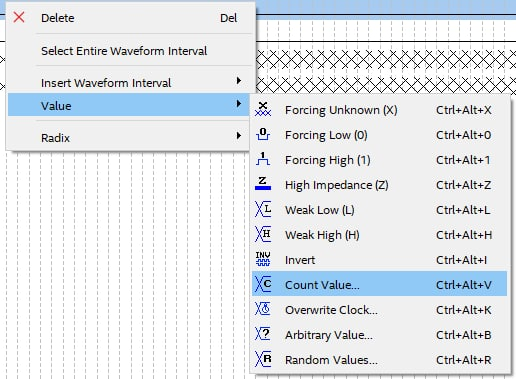
\includegraphics[width=12cm]{01_14}
    \caption{Установим \textbf{Count value} для каждого входа}
  \end{figure}

  \begin{figure}[H]
    \centering
    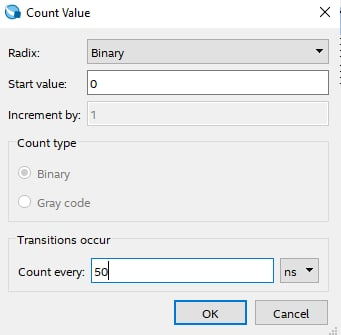
\includegraphics[width=6cm]{01_15}
    \caption{Для одного входа зададим поле \textbf{Count every} как 50ns, а для другого - 100ns}
  \end{figure}

  \begin{figure}[H]
    \centering
    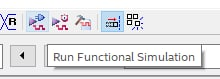
\includegraphics[width=6cm]{01_16}
    \caption{Запускаем функциональную симуляцию}
  \end{figure}

  \begin{figure}[H]
    \centering
    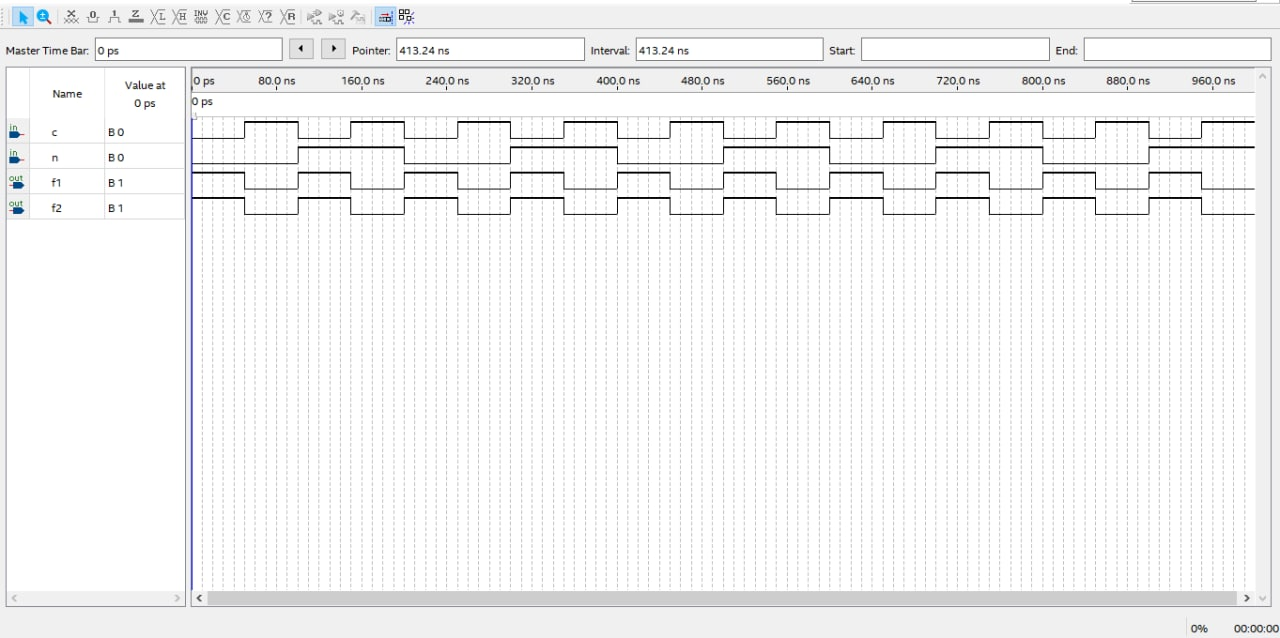
\includegraphics[width=12cm]{01_17}
    \caption{Видно, что уровни на логических выходах совпадают с таблицей истинности}
  \end{figure}

  \begin{figure}[H]
    \centering
    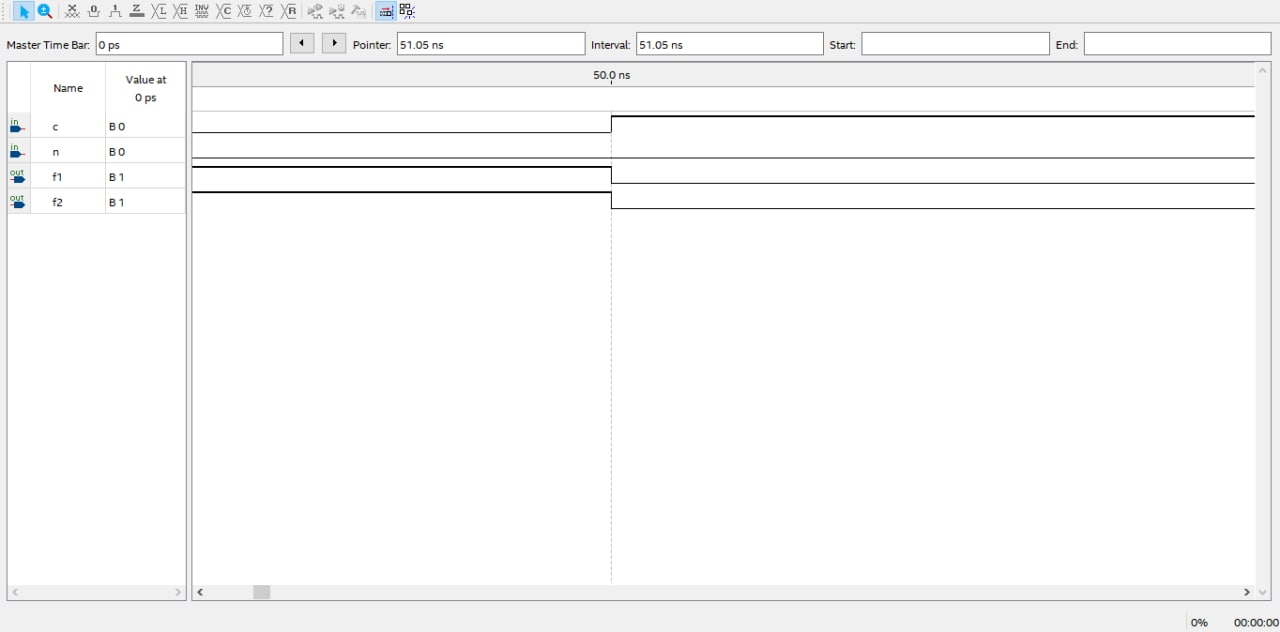
\includegraphics[width=12cm]{01_18}
    \caption{При временной симуляции видно, что задержки в работе схемы практически нет}
  \end{figure}

  \section{Часть 2}

  \begin{figure}[H]
    \centering
    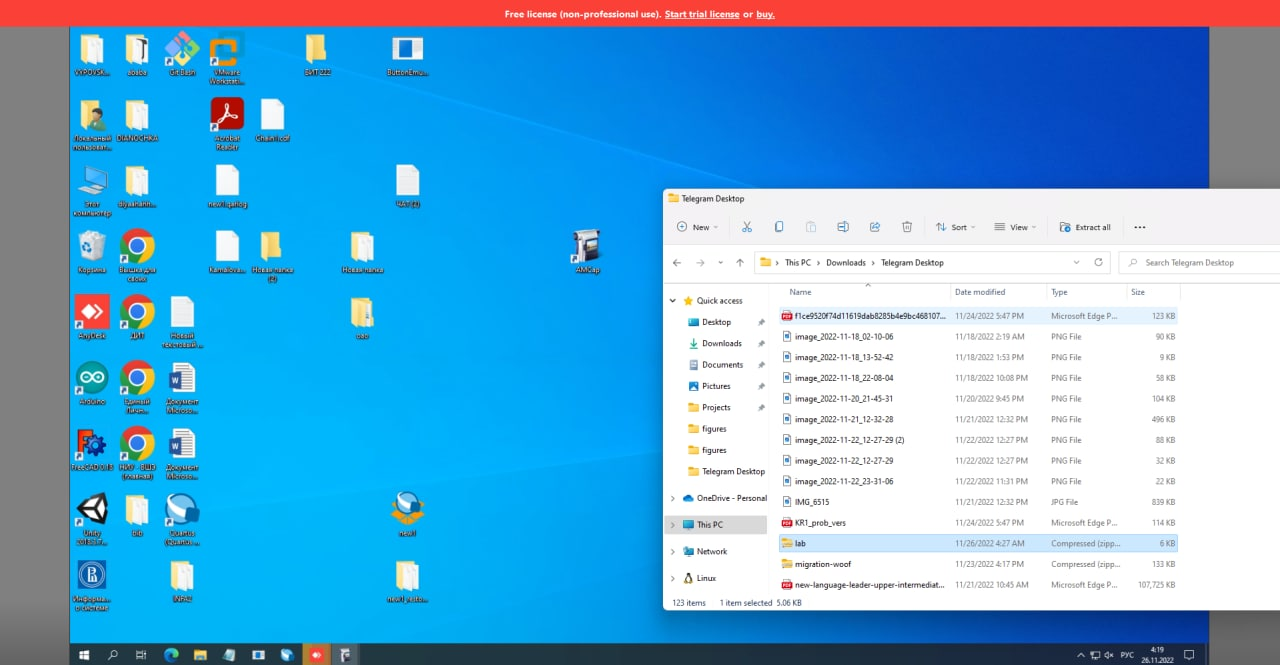
\includegraphics[width=12cm]{01_19}
    \caption{Подключимся к удаленному компьютера, с которого можно осуществить программирование стенда}
  \end{figure}

  \begin{figure}[H]
    \centering
    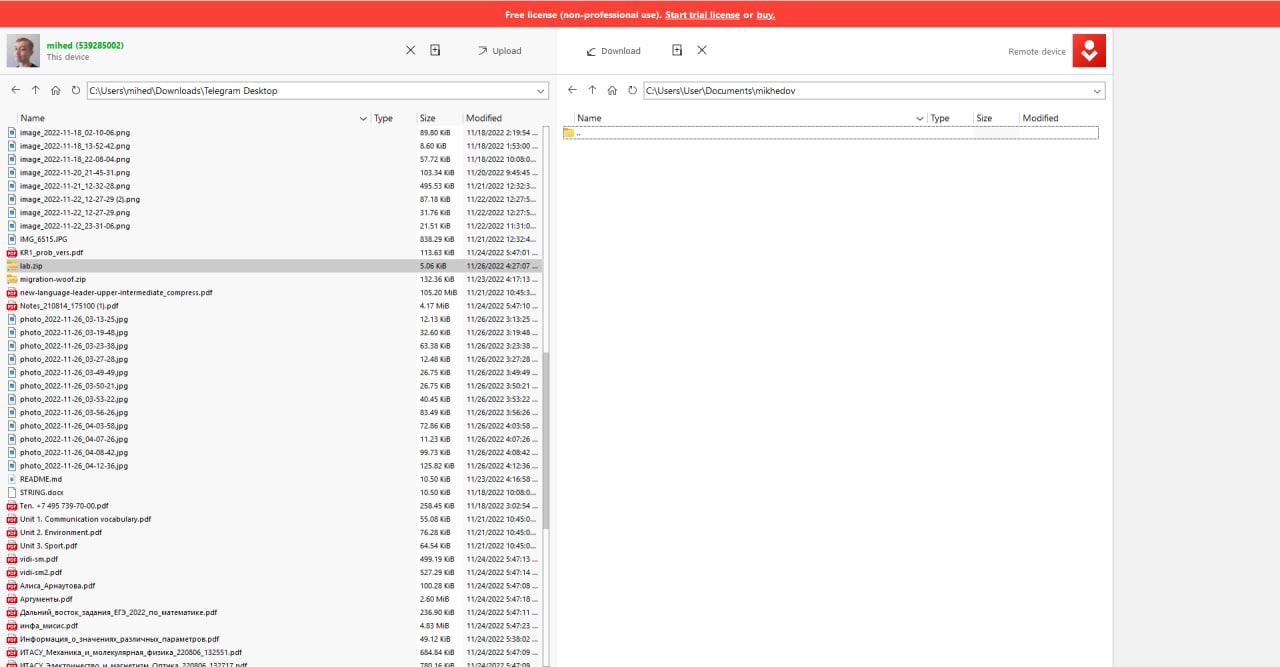
\includegraphics[width=12cm]{01_20}
    \caption{Перенесем на удаленный компьютер ранее созданные bdf и wvf файлы}
  \end{figure}

  \begin{figure}[H]
    \centering
    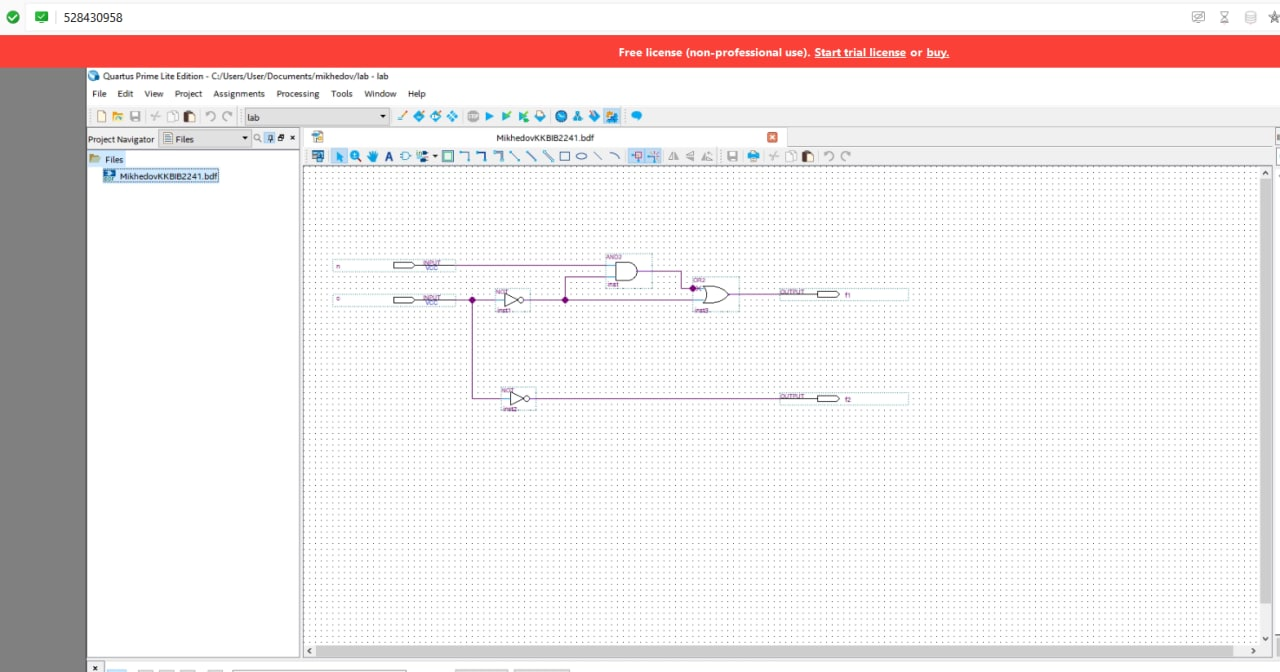
\includegraphics[width=12cm]{01_21}
    \caption{Откроем перенесенный проект}
  \end{figure}

  \begin{figure}[H]
    \centering
    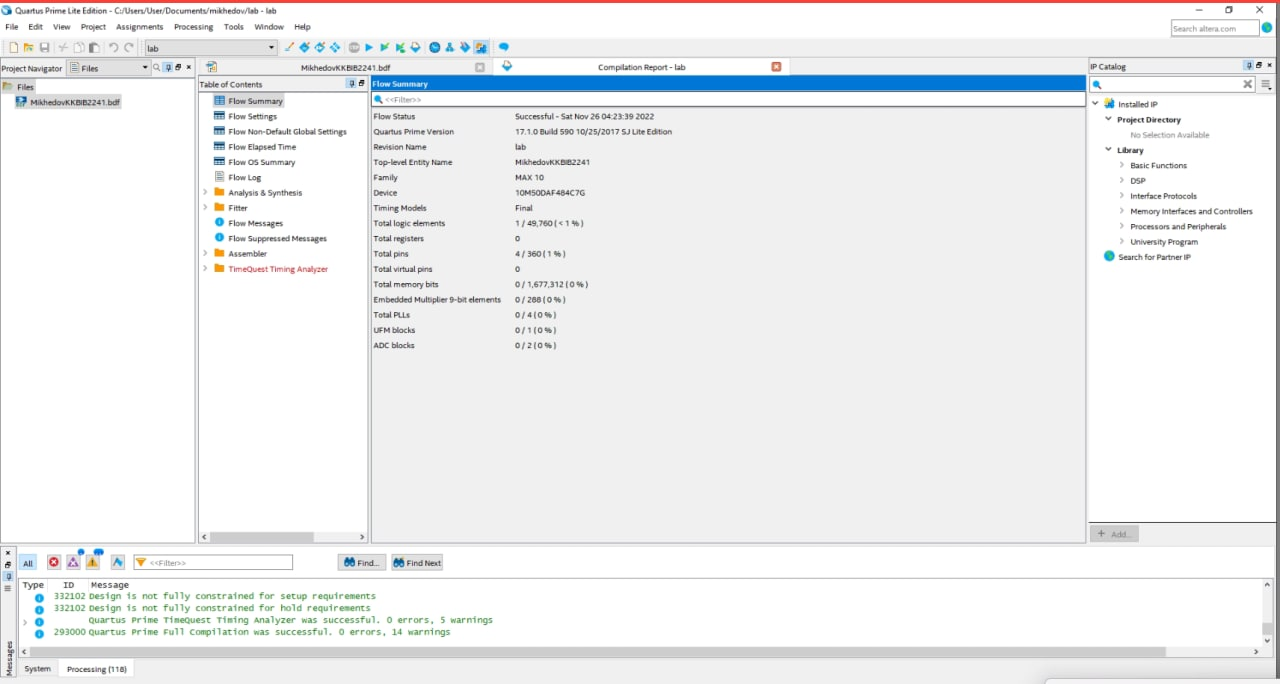
\includegraphics[width=12cm]{01_22}
    \caption{Выполним его компиляцию}
  \end{figure}

  \begin{figure}[H]
    \centering
    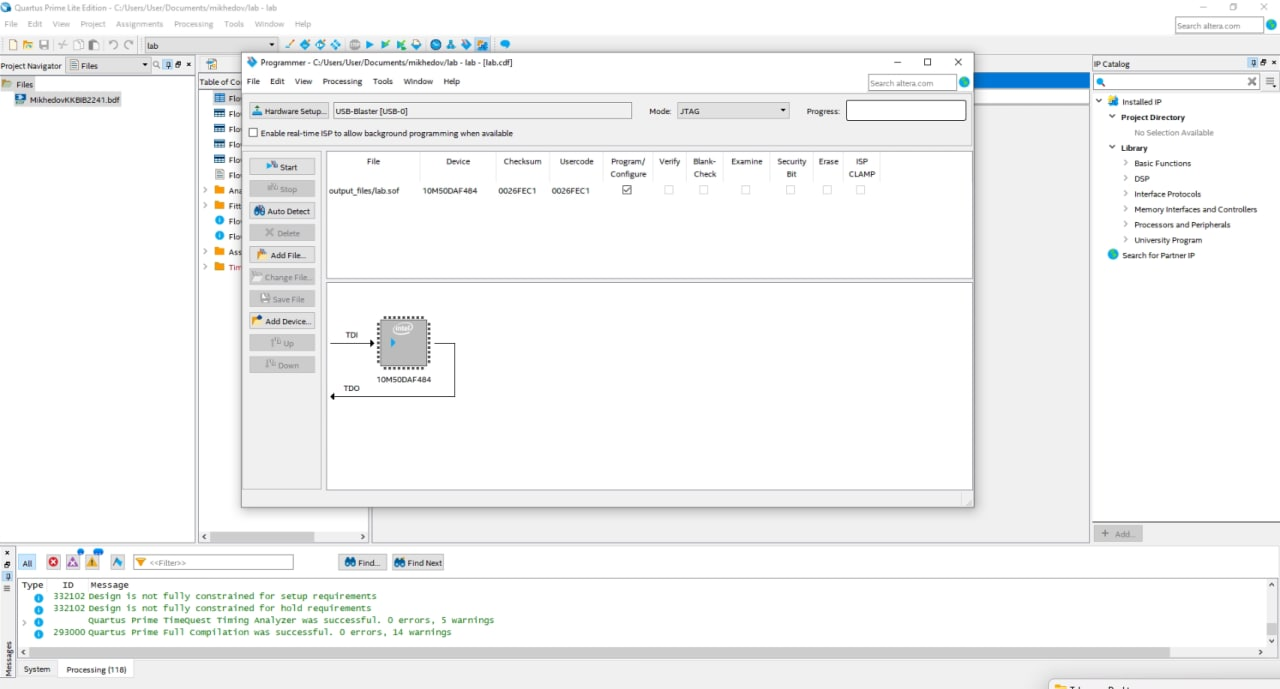
\includegraphics[width=12cm]{01_23}
    \caption{Откроем интерфейс для прошивки стенда}
  \end{figure}  

  \begin{figure}[H]
    \centering
    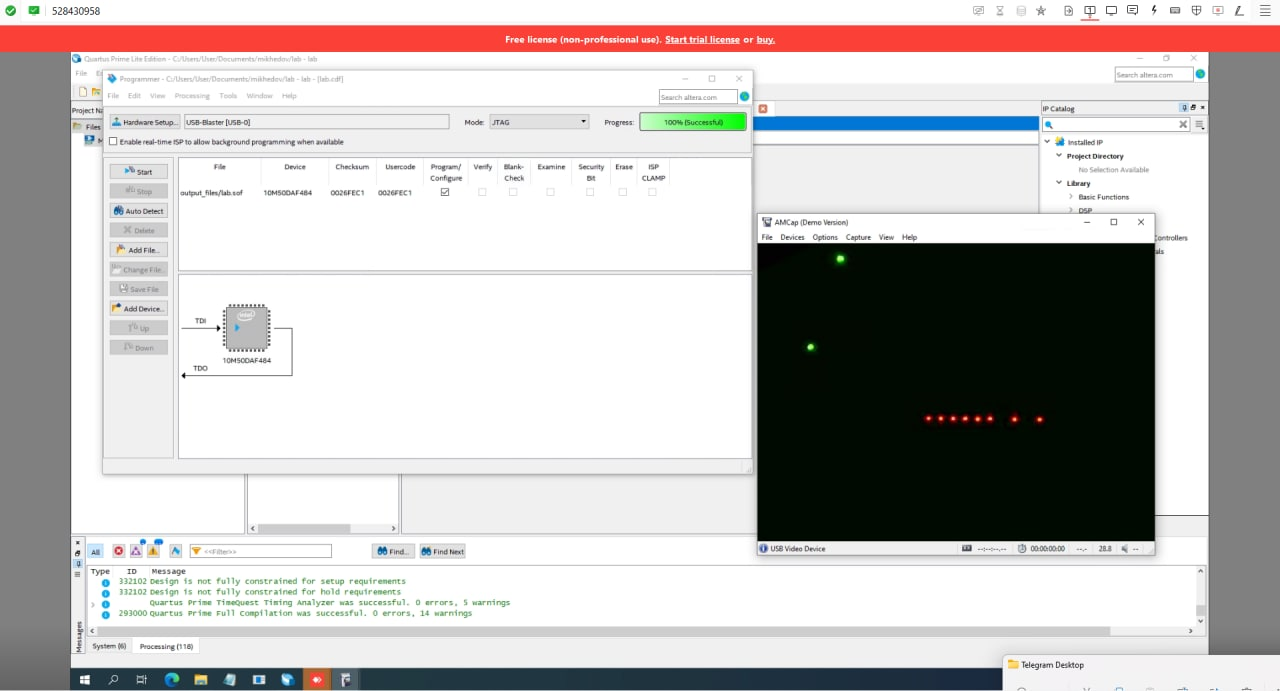
\includegraphics[width=12cm]{01_24}
    \caption{Загрузим программу на стенд и проверим его работоспособность}
  \end{figure}  

  \section{Контрольные вопросы}

  \begin{enumerate}
    \item {
        Панель управления сверху, окно выбора проектов, окно, где нужно создавать схему
    }
    \item {
        Зажать Ctrl и покрутить колесико мыши
    }
    \item {
        Orthogonal Node Tool выбирает средство для реализации элементов проводных
        соединений окна схемы, когда Orthogonal Bus Tool нужен для хранения множимого и
        множителя, их характеристик
    }
    \item {
        Run Functional Simulation проверяет только логику работы системы, а Run Timing Simulation
        позволяет также оценить и временные задержкти во время ее работы.
    }
    \item {
        Логическое И, ИЛИ, НЕ, И-НЕ, ИЛИ-НЕ, xor, НЕ-xor
    }
    \item {
        Waveform
    }
    \item {
        Чтобы удостовериться в корректности схемы и ее упрощенного варианта, оценить затраты на ее реализацию
    }
    \item {
        .bdf
    }
    \item {
        50 000
    }
    \item {
        Разъемы расширения, дисплей, переключатели, кнопки, светодиоды, датчик, 7-
        сегментный дисплей 64SD RAM, 16-битная шина данных
    }
    \item {
        64SD RAM, 16-битная шина данных
    }
    \item {
        4-bit resistor vga
    }
    \item {
        .bat
    }
    \item {
        $(a\land b\lor c\land d)\land (a \lor b) = \overline{\overline{a}\land\overline{b}} \land \overline{\overline{ab}\land\overline{cd}}$
    }
    \item {
        $(a\land b\lor c\land d)\land (a \lor b) = a\land b \lor a\land c\land d \lor b\land c\land d =
        \overline{\overline{a} \lor \overline{b}} \lor \overline{\overline{a} \lor \overline{c} \lor \overline{d}} \lor
        \overline{\overline{b} \lor \overline{c} \lor \overline{d}}$
    }
  \end{enumerate}

  \section{Вывод}

  В ходе данной лабораторной работы я научился основам работы с САПР Alter Quartus II, ознакомился
  с интерфейсом данного программного обеспечения, научился создавать и тестировать проекты
  как виртуально, так и на реальном оборудовании

\end{document}
